%----------------------------------------------------------------------------------------
%    PACKAGES AND THEMES
%----------------------------------------------------------------------------------------

\documentclass[aspectratio=169,xcolor=dvipsnames]{beamer}
\usetheme{SimpleDarkBlue}

\usepackage{hyperref}
\usepackage{graphicx} % Allows including images
\usepackage{booktabs} % Allows the use of \toprule, \midrule and \bottomrule in tables

%----------------------------------------------------------------------------------------
%    TITLE PAGE
%----------------------------------------------------------------------------------------

\title{Human-Benchmark}
\subtitle{3 Laboratorinis}

\author{Adrian, Arnas, Darius, Tadas}

\institute
{
    Matematikos ir informatikos fakultetas \\
    Vilniaus universitetas % Your institution for the title page
}
% \date{\today} % Date, can be changed to a custom date 

%----------------------------------------------------------------------------------------
%    PRESENTATION SLIDES
%----------------------------------------------------------------------------------------

\begin{document}

\begin{frame}
    % Print the title page as the first slide
    \titlepage
\end{frame}

\begin{frame}{Table of Contents}
    % Throughout your presentation, if you choose to use \section{} and \subsection{} commands, these will automatically be printed on this slide as an overview of your presentation
    \tableofcontents
\end{frame}

\section{UI Mockups}

\begin{frame}{UI Mockups Overview}
    \begin{itemize}
        \item The UI mockups cover all major chat functionalities:
        \begin{itemize}
            \item Global and room chat scopes
            \item Private and group chats
            \item Message management (send, edit, delete)
            \item File uploads and emoji selection
            \item Notifications and pinned messages
        \end{itemize}
        \item Main UI endpoints:
    \end{itemize}

    \begin{table}[]
        \centering
        \begin{tabular}{|l|l|}
            \hline
            \textbf{UI Section} & \textbf{Key Functionality} \\ \hline
            Global Chat         & Public messages, moderation \\ \hline
            Room Chat           & Game-room specific communication \\ \hline
            Private Chat        & 1:1 messaging with read receipts \\ \hline
            Group Chat          & Group communication with management \\ \hline
            Search Section      & Message search across all scopes \\ \hline
            Notifications       & Message alerts and system notifications \\ \hline
            Pinned Messages     & Important message preservation \\ \hline
        \end{tabular}
    \end{table}
\end{frame}

\begin{frame}{UI Mockup Examples}
    \begin{figure}
        \centering
        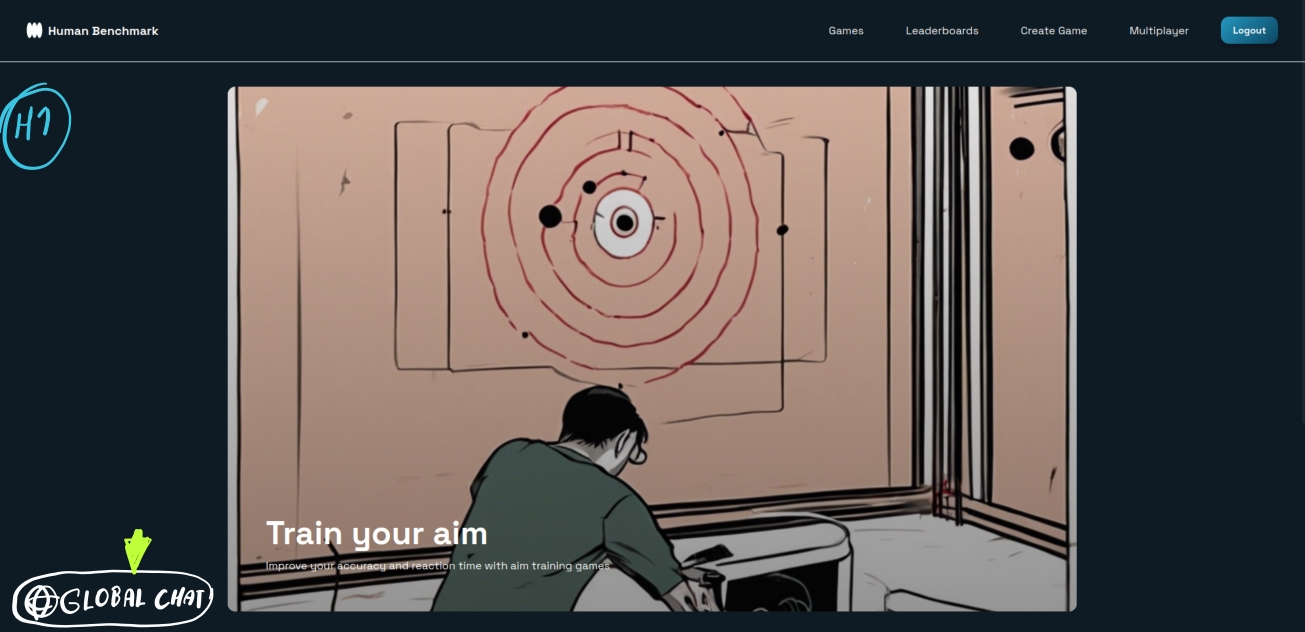
\includegraphics[width=0.3\textwidth]{images/UI/cropped/H1.png}
        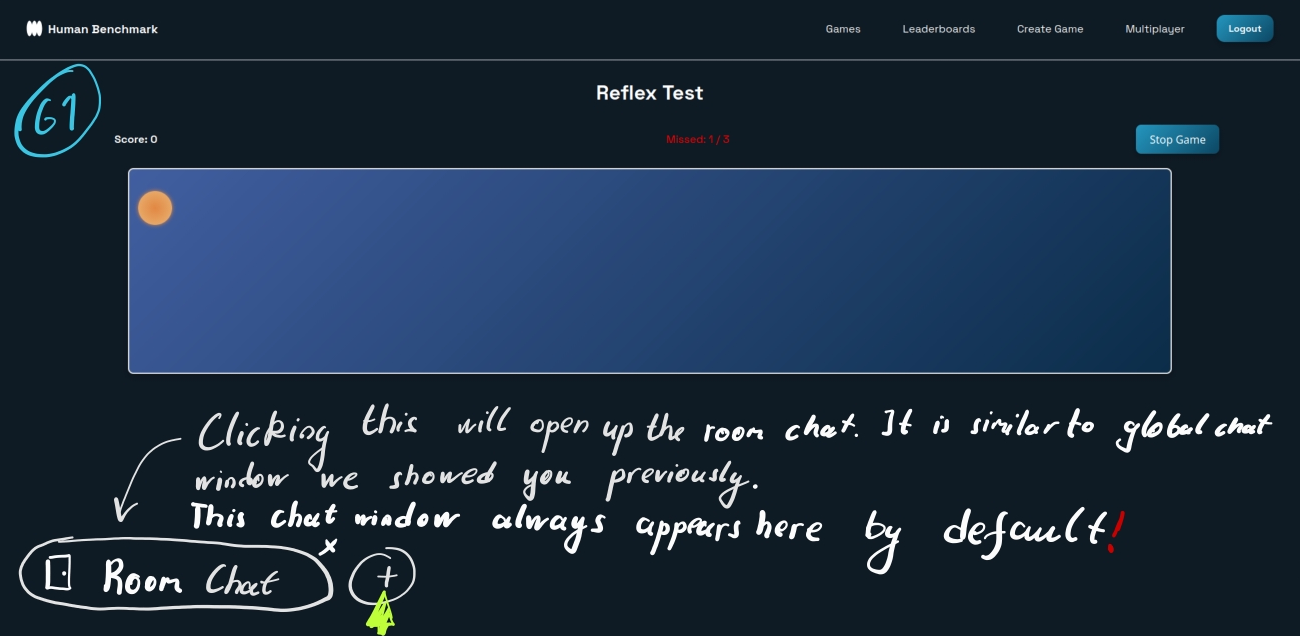
\includegraphics[width=0.3\textwidth]{images/UI/cropped/G1.png}
        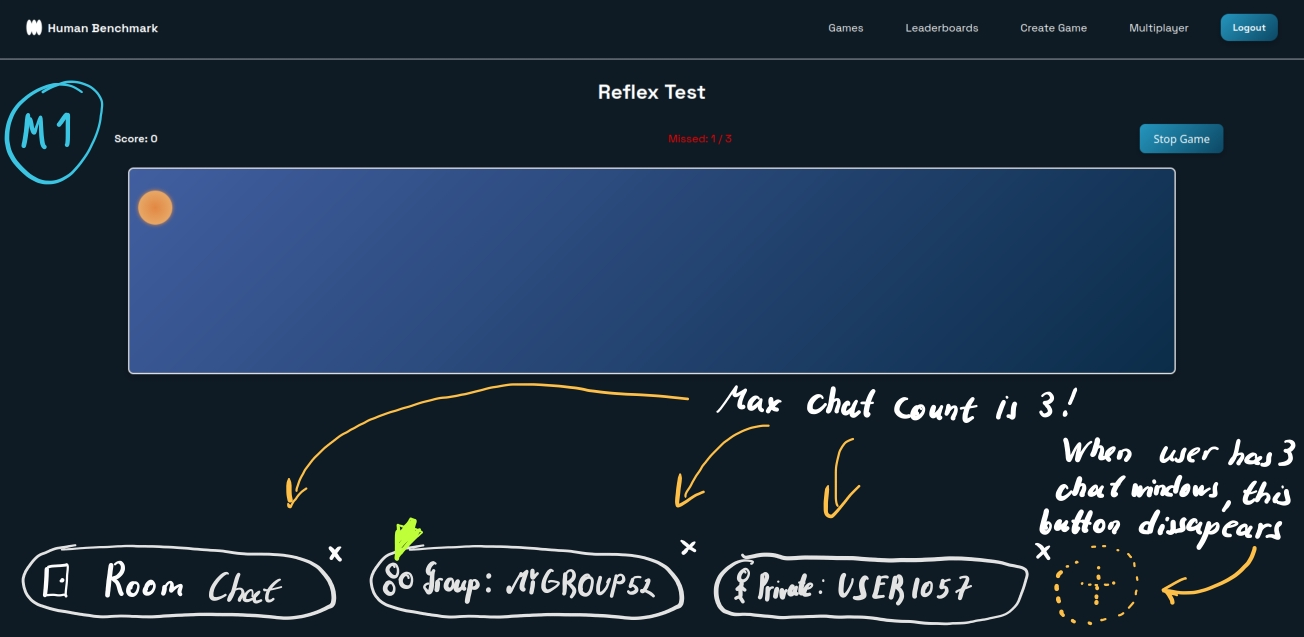
\includegraphics[width=0.3\textwidth]{images/UI/cropped/M1.png}
        \caption{Key UI mockups showing global chat, room chat, and multiple chat sections}
    \end{figure}
\end{frame}

\section{Domain Model Evolution}

\begin{frame}{Domain Model Development}
    \begin{itemize}
        \item Went through 8 iterations of refinement:
        \begin{enumerate}
            \item Initial noun extraction (v1)
            \item Removal of duplicates (v2)
            \item Added private chats and search (v3)
            \item Added UI components (v4)
            \item Refined search functionality (v5)
            \item Added editing panels (v6)
            \item Finalized relationships (v7)
            \item Added error handling (v8)
        \end{enumerate}
    \end{itemize}


\end{frame}

\begin{frame}{Domain Model Overview}
    \begin{figure}
        \centering
        
\includegraphics[width=0.45\textwidth]{images/domain1.png}
        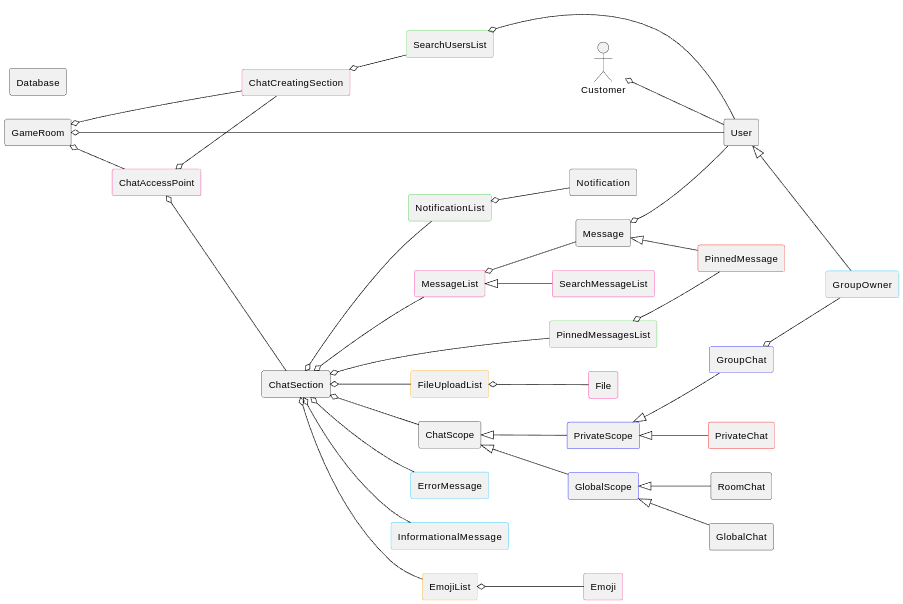
\includegraphics[width=0.45\textwidth]{images/domain8.png}
        \caption{Initial (left) vs Final (right) domain model versions}
    \end{figure}
\end{frame}

\section{Use Cases}

\begin{frame}{Use Case Overview}
    \begin{itemize}
        \item Organized into 6 packages:
        \begin{itemize}
            \item Core Chat Functionality
            \item Message Management
            \item Chat Management
            \item Notification System
            \item UI Interactions
            \item Administrative
        \end{itemize}
        \item Average of 2-3 alternative scenarios per use case
        \item Detailed error handling for all operations
    \end{itemize}
\end{frame}

\begin{frame}{Use Case Package Diagram}
    \begin{figure}
        \centering
        
\includegraphics[width=0.7\textwidth]{images/packageDiagram.png}
        \caption{Use Case Package Diagram}
    \end{figure}
\end{frame}

\begin{frame}{Key Use Case Diagrams}
    \begin{figure}
        \centering
        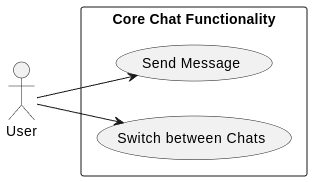
\includegraphics[width=0.25\textwidth]{images/UseCaseDiagrams/corChat.png}
        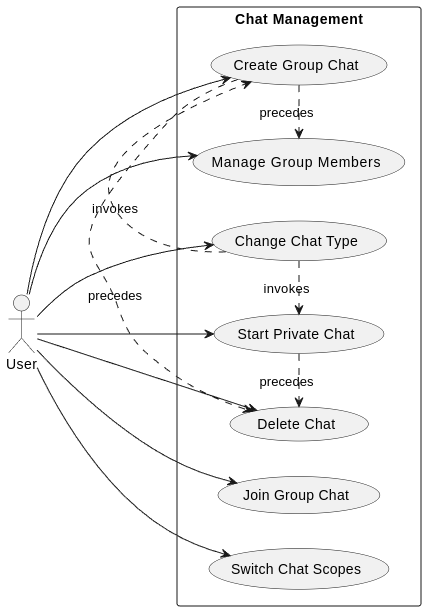
\includegraphics[width=0.25\textwidth]{images/UseCaseDiagrams/chatMan.png}
        \caption{Core Chat (left) and Chat Management (right) use cases}
    \end{figure}
\end{frame}

\begin{frame}{Use Case Characteristics}
    \begin{itemize}
        \item Comprehensive coverage of:
        \begin{itemize}
            \item Normal operation flows
            \item Error conditions
            \item Edge cases
        \end{itemize}
        \item Example statistics:
        \begin{itemize}
            \item 22 primary use cases
            \item 58 alternative flows
            \item 70+ requirements traced
        \end{itemize}
        \item Focus on real-world scenarios:
        \begin{itemize}
            \item Message validation
            \item Chat management
            \item User notifications
        \end{itemize}
    \end{itemize}
\end{frame}



\end{document}
